% Options for packages loaded elsewhere
\PassOptionsToPackage{unicode}{hyperref}
\PassOptionsToPackage{hyphens}{url}
\PassOptionsToPackage{dvipsnames,svgnames,x11names}{xcolor}
%
\documentclass[
  11pt,
  a4paper,
]{article}

\usepackage{amsmath,amssymb}
\usepackage{setspace}
\usepackage{iftex}
\ifPDFTeX
  \usepackage[T1]{fontenc}
  \usepackage[utf8]{inputenc}
  \usepackage{textcomp} % provide euro and other symbols
\else % if luatex or xetex
  \usepackage{unicode-math}
  \defaultfontfeatures{Scale=MatchLowercase}
  \defaultfontfeatures[\rmfamily]{Ligatures=TeX,Scale=1}
\fi
\usepackage{lmodern}
\ifPDFTeX\else  
    % xetex/luatex font selection
    \setmainfont[]{Palatino Linotype}
\fi
% Use upquote if available, for straight quotes in verbatim environments
\IfFileExists{upquote.sty}{\usepackage{upquote}}{}
\IfFileExists{microtype.sty}{% use microtype if available
  \usepackage[]{microtype}
  \UseMicrotypeSet[protrusion]{basicmath} % disable protrusion for tt fonts
}{}
\makeatletter
\@ifundefined{KOMAClassName}{% if non-KOMA class
  \IfFileExists{parskip.sty}{%
    \usepackage{parskip}
  }{% else
    \setlength{\parindent}{0pt}
    \setlength{\parskip}{6pt plus 2pt minus 1pt}}
}{% if KOMA class
  \KOMAoptions{parskip=half}}
\makeatother
\usepackage{xcolor}
\usepackage[top=2.4cm,bottom=2.4cm,left=2.5cm,right=2.5cm]{geometry}
\setlength{\emergencystretch}{3em} % prevent overfull lines
\setcounter{secnumdepth}{-\maxdimen} % remove section numbering


\providecommand{\tightlist}{%
  \setlength{\itemsep}{0pt}\setlength{\parskip}{0pt}}\usepackage{longtable,booktabs,array}
\usepackage{calc} % for calculating minipage widths
% Correct order of tables after \paragraph or \subparagraph
\usepackage{etoolbox}
\makeatletter
\patchcmd\longtable{\par}{\if@noskipsec\mbox{}\fi\par}{}{}
\makeatother
% Allow footnotes in longtable head/foot
\IfFileExists{footnotehyper.sty}{\usepackage{footnotehyper}}{\usepackage{footnote}}
\makesavenoteenv{longtable}
\usepackage{graphicx}
\makeatletter
\def\maxwidth{\ifdim\Gin@nat@width>\linewidth\linewidth\else\Gin@nat@width\fi}
\def\maxheight{\ifdim\Gin@nat@height>\textheight\textheight\else\Gin@nat@height\fi}
\makeatother
% Scale images if necessary, so that they will not overflow the page
% margins by default, and it is still possible to overwrite the defaults
% using explicit options in \includegraphics[width, height, ...]{}
\setkeys{Gin}{width=\maxwidth,height=\maxheight,keepaspectratio}
% Set default figure placement to htbp
\makeatletter
\def\fps@figure{htbp}
\makeatother

\usepackage{booktabs}
\usepackage{longtable}
\usepackage{array}
\usepackage{multirow}
\usepackage{wrapfig}
\usepackage{float}
\usepackage{colortbl}
\usepackage{pdflscape}
\usepackage{tabu}
\usepackage{threeparttable}
\usepackage{threeparttablex}
\usepackage[normalem]{ulem}
\usepackage{makecell}
\usepackage{xcolor}
\usepackage{caption}
\usepackage{anyfontsize}
\makeatletter
\@ifpackageloaded{tcolorbox}{}{\usepackage[skins,breakable]{tcolorbox}}
\@ifpackageloaded{fontawesome5}{}{\usepackage{fontawesome5}}
\definecolor{quarto-callout-color}{HTML}{909090}
\definecolor{quarto-callout-note-color}{HTML}{0758E5}
\definecolor{quarto-callout-important-color}{HTML}{CC1914}
\definecolor{quarto-callout-warning-color}{HTML}{EB9113}
\definecolor{quarto-callout-tip-color}{HTML}{00A047}
\definecolor{quarto-callout-caution-color}{HTML}{FC5300}
\definecolor{quarto-callout-color-frame}{HTML}{acacac}
\definecolor{quarto-callout-note-color-frame}{HTML}{4582ec}
\definecolor{quarto-callout-important-color-frame}{HTML}{d9534f}
\definecolor{quarto-callout-warning-color-frame}{HTML}{f0ad4e}
\definecolor{quarto-callout-tip-color-frame}{HTML}{02b875}
\definecolor{quarto-callout-caution-color-frame}{HTML}{fd7e14}
\makeatother
\makeatletter
\@ifpackageloaded{caption}{}{\usepackage{caption}}
\AtBeginDocument{%
\ifdefined\contentsname
  \renewcommand*\contentsname{Table of contents}
\else
  \newcommand\contentsname{Table of contents}
\fi
\ifdefined\listfigurename
  \renewcommand*\listfigurename{List of Figures}
\else
  \newcommand\listfigurename{List of Figures}
\fi
\ifdefined\listtablename
  \renewcommand*\listtablename{List of Tables}
\else
  \newcommand\listtablename{List of Tables}
\fi
\ifdefined\figurename
  \renewcommand*\figurename{Figure}
\else
  \newcommand\figurename{Figure}
\fi
\ifdefined\tablename
  \renewcommand*\tablename{Table}
\else
  \newcommand\tablename{Table}
\fi
}
\@ifpackageloaded{float}{}{\usepackage{float}}
\floatstyle{ruled}
\@ifundefined{c@chapter}{\newfloat{codelisting}{h}{lop}}{\newfloat{codelisting}{h}{lop}[chapter]}
\floatname{codelisting}{Listing}
\newcommand*\listoflistings{\listof{codelisting}{List of Listings}}
\makeatother
\makeatletter
\makeatother
\makeatletter
\@ifpackageloaded{caption}{}{\usepackage{caption}}
\@ifpackageloaded{subcaption}{}{\usepackage{subcaption}}
\makeatother
\makeatletter
\@ifpackageloaded{sidenotes}{}{\usepackage{sidenotes}}
\@ifpackageloaded{marginnote}{}{\usepackage{marginnote}}
\makeatother

\ifLuaTeX
  \usepackage{selnolig}  % disable illegal ligatures
\fi
\usepackage{bookmark}

\IfFileExists{xurl.sty}{\usepackage{xurl}}{} % add URL line breaks if available
\urlstyle{same} % disable monospaced font for URLs
\hypersetup{
  pdftitle={Survey Experiment},
  pdfauthor={Isaiah},
  pdfkeywords={Election Workers, Poll workers, Veterans, Public
opinion, Election administration},
  colorlinks=true,
  linkcolor={blue},
  filecolor={Maroon},
  citecolor={Blue},
  urlcolor={Blue},
  pdfcreator={LaTeX via pandoc}}

%% CAPTIONS
\usepackage{caption}
\DeclareCaptionStyle{italic}[justification=centering]
 {labelfont={bf},textfont={it},labelsep=colon}
\captionsetup[figure]{style=italic,format=hang,singlelinecheck=true}
\captionsetup[table]{style=italic,format=hang,singlelinecheck=true}

%% FONT
% \usepackage{bera}
% \usepackage[charter]{mathdesign}
% \usepackage[scale=0.9]{sourcecodepro}
% \usepackage[lf,t]{FiraSans}
\usepackage{fontawesome}

%% HEADERS AND FOOTERS
\usepackage{fancyhdr}
\pagestyle{fancy}
\rfoot{\Large\sffamily\raisebox{-0.1cm}{\textbf{\thepage}}}
\makeatletter
\lhead{\textsf{\expandafter{\@title}}}
\makeatother
\rhead{}
\cfoot{}
\setlength{\headheight}{15pt}
\renewcommand{\headrulewidth}{0.4pt}
\renewcommand{\footrulewidth}{0.4pt}
\fancypagestyle{plain}{%
\fancyhf{} % clear all header and footer fields
\fancyfoot[C]{\sffamily\thepage} % except the center
\renewcommand{\headrulewidth}{0pt}
\renewcommand{\footrulewidth}{0pt}}

%% MATHS
\usepackage{bm,amsmath}
\allowdisplaybreaks

%% GRAPHICS
\makeatletter
\def\fps@figure{htbp}
\makeatother
\setcounter{topnumber}{2}
\setcounter{bottomnumber}{2}
\setcounter{totalnumber}{4}
\renewcommand{\topfraction}{0.85}
\renewcommand{\bottomfraction}{0.85}
\renewcommand{\textfraction}{0.15}
\renewcommand{\floatpagefraction}{0.8}

%% SECTION TITLES
\usepackage[compact,sf,bf]{titlesec}
\titleformat*{\section}{\Large\sf\bfseries\color[rgb]{0.7,0,0}}
\titleformat*{\subsection}{\large\sf\bfseries\color[rgb]{0.7,0,0}}
\titleformat*{\subsubsection}{\sf\bfseries\color[rgb]{0.7,0,0}}
\titlespacing{\section}{0pt}{2ex}{.5ex}
\titlespacing{\subsection}{0pt}{1.5ex}{0ex}
\titlespacing{\subsubsection}{0pt}{.5ex}{0ex}


%% BIBLIOGRAPHY.

\makeatletter
\@ifpackageloaded{biblatex}{
\ExecuteBibliographyOptions{bibencoding=utf8,minnames=1,maxnames=3, maxbibnames=99,dashed=false,terseinits=true,giveninits=true,uniquename=false,uniquelist=false,doi=false, isbn=false,url=true,sortcites=false}
\DeclareFieldFormat{url}{\texttt{\url{#1}}}
\DeclareFieldFormat[article]{pages}{#1}
\DeclareFieldFormat[inproceedings]{pages}{\lowercase{pp.}#1}
\DeclareFieldFormat[incollection]{pages}{\lowercase{pp.}#1}
\DeclareFieldFormat[article]{volume}{\mkbibbold{#1}}
\DeclareFieldFormat[article]{number}{\mkbibparens{#1}}
\DeclareFieldFormat[article]{title}{\MakeCapital{#1}}
\DeclareFieldFormat[article]{url}{}
\DeclareFieldFormat[inproceedings]{title}{#1}
\DeclareFieldFormat{shorthandwidth}{#1}
\usepackage{xpatch}
\xpatchbibmacro{volume+number+eid}{\setunit*{\adddot}}{}{}{}
% Remove In: for an article.
\renewbibmacro{in:}{%
  \ifentrytype{article}{}{%
  \printtext{\bibstring{in}\intitlepunct}}}
\AtEveryBibitem{\clearfield{month}}
\AtEveryCitekey{\clearfield{month}}
\DeclareDelimFormat[cbx@textcite]{nameyeardelim}{\addspace}
\renewcommand*{\finalnamedelim}{\addspace\&\space}
}{}
\makeatother

%% PAGE BREAKING to avoid widows and orphans
\clubpenalty = 2000
\widowpenalty = 2000
\usepackage{microtype}
% Placement of logos

\RequirePackage[absolute,overlay]{textpos}
\setlength{\TPHorizModule}{1cm}
\setlength{\TPVertModule}{1cm}
\def\placefig#1#2#3#4{\begin{textblock}{.1}(#1,#2)\rlap{\includegraphics[#3]{#4}}\end{textblock}}

% Title and date

\title{Survey Experiment}
\date{2024-9-12}

\def\Date{\number\day}
\def\Month{\ifcase\month\or
 January\or February\or March\or April\or May\or June\or
 July\or August\or September\or October\or November\or December\fi}
\def\Year{\number\year}

%%%% PAGE STYLE FOR FRONT PAGE OF REPORTS

\makeatletter
\def\organization#1{\gdef\@organization{#1}}
\def\telephone#1{\gdef\@telephone{#1}}
\def\email#1{\gdef\@email{#1}}
\makeatother
  \organization{}

  \def\name{Center for Democracy and Civic Engagement}
% 
  \telephone{(410) 903 6911}
% 
  \email{ssnovey@umd.edu}

\def\webaddress{\url{https://cdce.umd.edu/}}
\def\abn{12 377 614 012}
\def\extraspace{\vspace*{1.6cm}}
\makeatletter
\def\contactdetails{\faicon{phone} & \@telephone \\
                    \faicon{envelope} & \@email}
\makeatother

\usepackage[absolute,overlay]{textpos}
\setlength{\TPHorizModule}{1cm}
\setlength{\TPVertModule}{1cm}

%%%% FRONT PAGE OF REPORTS

% \def\reporttype{Report}

\long\def\front#1#2#3{
\newpage
% \begin{textblock}{7}(12.7,28.2)\hfill
% 
\includegraphics[height=4cm]{umd_logo2}~~~
% \end{textblock}
\begin{singlespacing}
\thispagestyle{empty}
\vspace*{-1.4cm}
\hspace*{-1.4cm}
\hbox to 16cm{
  \hbox to 6.5cm{\vbox to 14cm{\vbox to 25cm{
    
\includegraphics[width=6.6cm]{CDCE}
    \vfill
    
\includegraphics[width=5cm]{umd_logo2}
    \vspace{0.4cm}
    \par
    \parbox{6.3cm}{\raggedright
      \sf\color[rgb]{0.70,0.00,0.00}
      {\large\textbf{\name}}\par
      \vspace{.7cm}
      \tabcolsep=0.12cm\sf\small
      \begin{tabular}{@{}ll@{}}\contactdetails
      \end{tabular}
    }
  }\vss}\hss}
  \hspace*{0.2cm}
  \hbox to 1cm{\vbox to 14cm{\rule{1pt}{26.8cm}\vss}\hss\hfill}
  \hbox to 10cm{\vbox to 14cm{\vbox to 25cm{
      \vspace*{3cm}\sf\raggedright
      \parbox{10cm}{\sf\raggedright\baselineskip=1.2cm
         \fontsize{24.88}{30}\color[rgb]{0.70,0.00,0.00}\sf\textbf{#1}}
      \par
      \vfill
      \large
      \vbox{\parskip=0.8cm #2}\par
      \vspace*{2cm}\par
      % \reporttype\\[0.3cm]
      % \hbox{#3}%\\[2cm]\
      % \vspace*{1cm}
      %{\large\sf\textbf{\Date~\Month~\Year}}
   }\vss}
  }}
\end{singlespacing}
\newpage
}

\makeatletter
\def\maketitle{\front{\expandafter{\@title}}{\@author}{\@organization}}
\makeatother

% Authors

\author{\sf{\Large\textbf{Isaiah} \\[0.5cm]}}
%\lfoot{\sf Isaiah: 2024-9-12}
\begin{document}
\maketitle


\setstretch{1.5}
\subsection{Key Questions}\label{key-questions}

The following presents some key results from the survey experiment.

\subsubsection{Q19}\label{q19}

\marginnote{\begin{footnotesize}

\begingroup
\setlength{\LTpost}{0mm}
\begin{longtable}{lllll}
\caption{Confidence vote counts will be accurate in Maricopa County, AZ by
Experiment Condition}\tabularnewline

\toprule
 & \multicolumn{4}{c}{{\bfseries Q19. Vote Count Confidence for Maricopa County, AZ}\textsuperscript{\textit{1}}} \\ 
\cmidrule(lr){2-5}
Group & {\bfseries Not at all confident} & {\bfseries Not too confident} & {\bfseries Somewhat confident} & {\bfseries Very confident} \\ 
\midrule\addlinespace[2.5pt]
Control & 3.8 (24) & 17.1 (107) & 49.2 (307) & 29.8 (186) \\ 
Treatment & 3.9 (25) & 12.7  (81) & 46.6 (298) & 36.8 (235) \\ 
\bottomrule
\end{longtable}
\begin{minipage}{\linewidth}
Table reflects row percentages. NAs omitted\\
\textsuperscript{\textit{1}}Q19. How confident are you that votes in Maricopa County, AZ will be counted as voters intend in the elections this November?\\
\end{minipage}
\endgroup

Confidence in Accurate Vote Count by Experiment Condition

\end{footnotesize}}

\begin{figure}[H]

{\centering 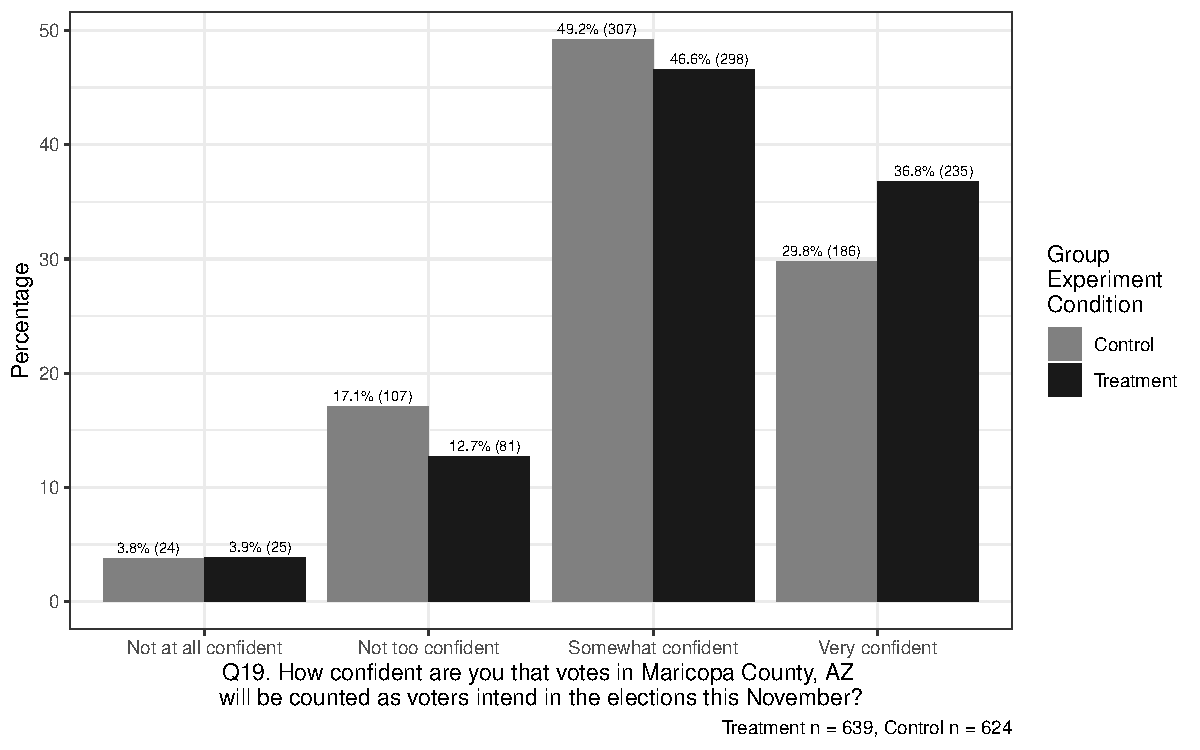
\includegraphics{index_files/figure-pdf/unnamed-chunk-3-1.pdf}

}

\caption{Confidence in Accurate Vote Count by Experiment Condition}

\end{figure}%

\subsubsection{Q22}\label{q22}

\marginnote{\begin{footnotesize}

\begingroup
\setlength{\LTpost}{0mm}
\begin{longtable}{lllll}
\caption{Q22. Confidence in Fair Voting Process by Experiment Condition in
Maricopa County, AZ by Experiment Condition}\tabularnewline

\toprule
 & \multicolumn{4}{c}{{\bfseries Q22. Confidence in Fair Voting Process for Maricopa County, AZ}\textsuperscript{\textit{1}}} \\ 
\cmidrule(lr){2-5}
Group & {\bfseries Not at all confident} & {\bfseries Not too confident} & {\bfseries Somewhat confident} & {\bfseries Very confident} \\ 
\midrule\addlinespace[2.5pt]
Control & 4.8 (30) & 18.9 (118) & 45.2 (282) & 31.1 (194) \\ 
Treatment & 4.2 (27) & 12.2  (78) & 46.3 (296) & 37.2 (238) \\ 
\bottomrule
\end{longtable}
\begin{minipage}{\linewidth}
Table reflects row percentages. NAs omitted\\
\textsuperscript{\textit{1}}Q22.How confident are you that the voting process will be fair in Maricopa County, AZ?\\
\end{minipage}
\endgroup

Confidence in Fair Voting Process by Experiment Condition

\end{footnotesize}}

\begin{figure}[H]

{\centering 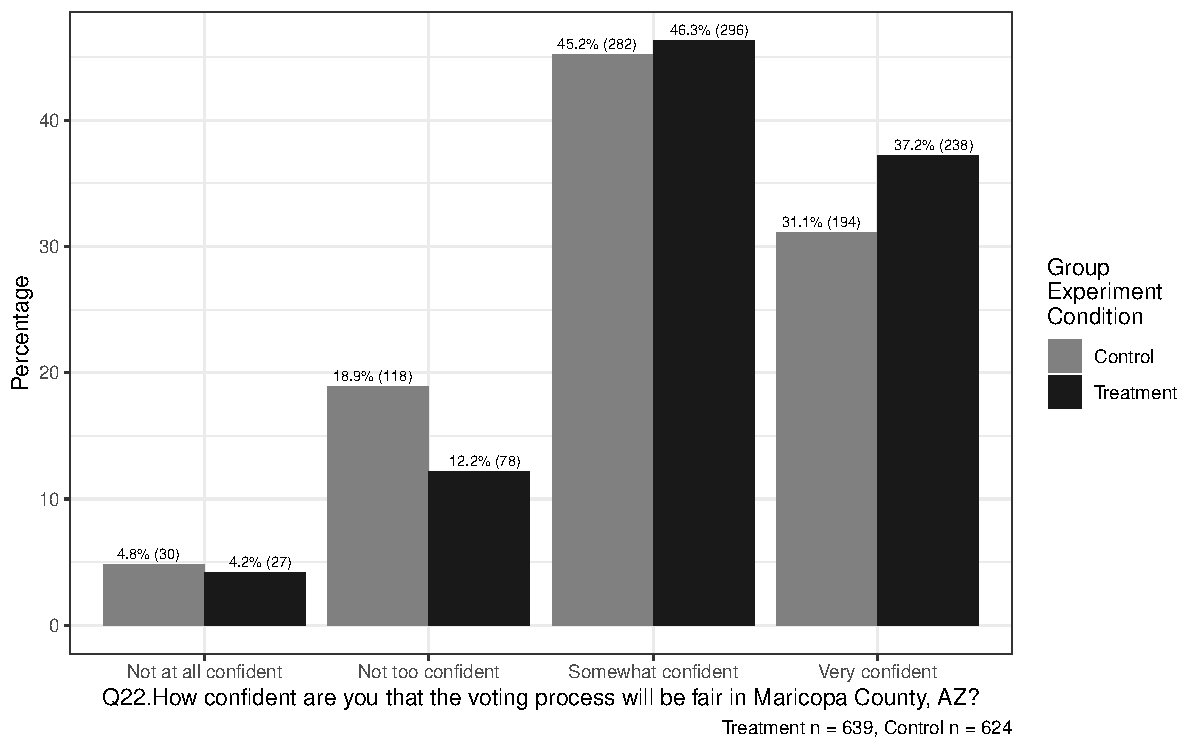
\includegraphics{index_files/figure-pdf/unnamed-chunk-4-1.pdf}

}

\caption{Confidence in Fair Voting Process by Experiment Condition}

\end{figure}%

\subsubsection{Q25}\label{q25}

\marginnote{\begin{footnotesize}

\begingroup
\setlength{\LTpost}{0mm}
\begin{longtable}{lllll}
\caption{Concern for violence, threats, or voter intimidation in Maricopa County,
AZ by Experiment Condition}\tabularnewline

\toprule
 & \multicolumn{4}{c}{{\bfseries Concern for violence, threats, or voter intimidation in Maricopa County, AZ}\textsuperscript{\textit{1}}} \\ 
\cmidrule(lr){2-5}
Group & {\bfseries Not at all concerned} & {\bfseries Not too concerned} & {\bfseries Somewhat concerned} & {\bfseries Very concerned} \\ 
\midrule\addlinespace[2.5pt]
Control & 12.8  (80) & 34.0 (212) & 41.0 (256) & 12.2 (76) \\ 
Treatment & 16.1 (103) & 38.5 (246) & 34.1 (218) & 11.3 (72) \\ 
\bottomrule
\end{longtable}
\begin{minipage}{\linewidth}
Table reflects row percentages. NAs omitted\\
\textsuperscript{\textit{1}}Q25. Thinking about Maricopa County, AZ, how concerned should voters feel 
about potential violence, 
threats of violence, or intimidation while voting in person at their local polling place?\\
\end{minipage}
\endgroup

Concern for violence, threats, or voter intimidation in Maricopa County,
AZ by Experiment Condition

\end{footnotesize}}

\begin{figure}[H]

{\centering 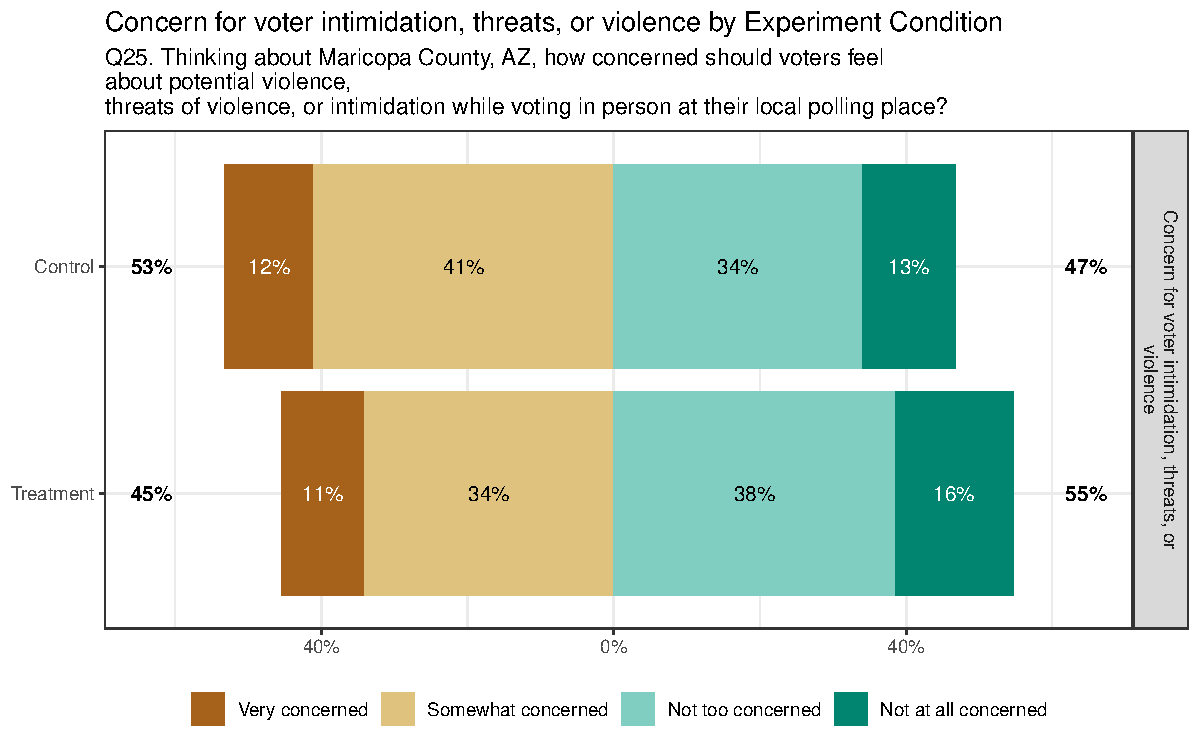
\includegraphics{index_files/figure-pdf/unnamed-chunk-5-1.pdf}

}

\caption{Concern for violence, threats, or voter intimidation in
Maricopa County, AZ by Experiment Condition}

\end{figure}%

\subsubsection{Q26}\label{q26}

\begin{figure}[H]

{\centering 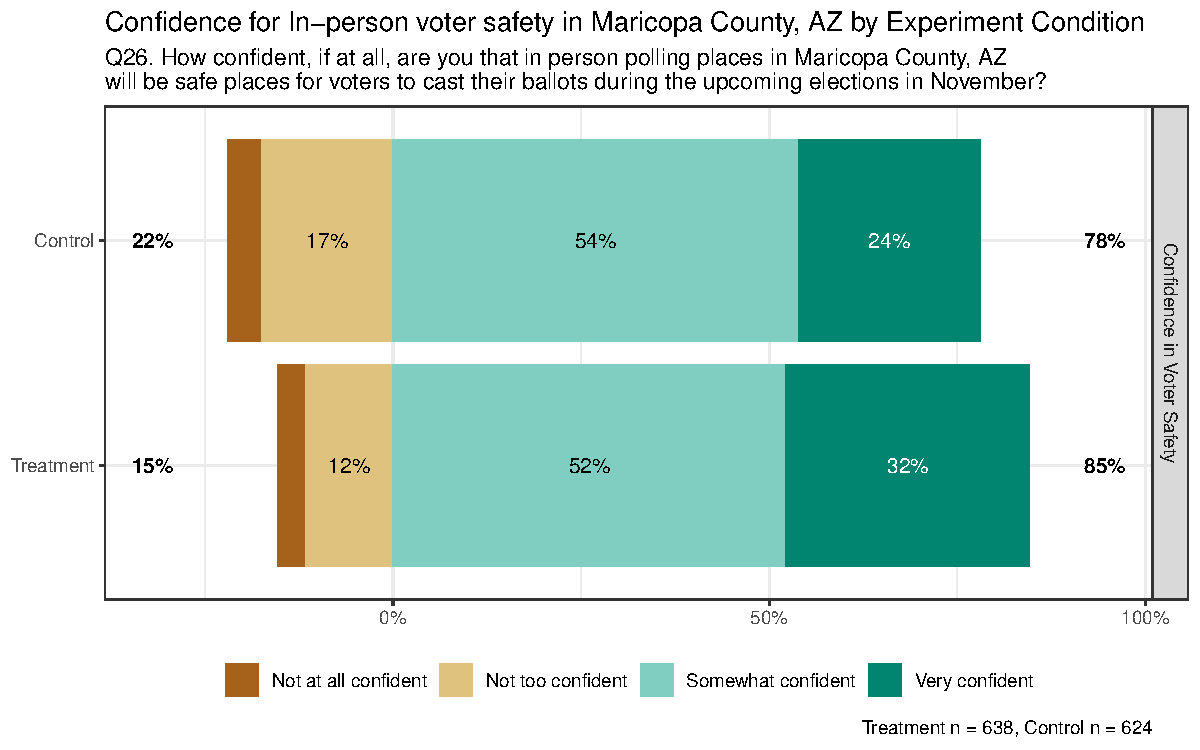
\includegraphics{index_files/figure-pdf/unnamed-chunk-6-1.pdf}

}

\caption{In-person voter safety in Maricopa County, AZ by Experiment
Condition}

\end{figure}%

\marginnote{\begin{footnotesize}

\begingroup
\setlength{\LTpost}{0mm}
\begin{longtable}{lllll}
\caption{Q26. In-person voter safety in Maricopa County, AZ by Experiment
Condition}\tabularnewline

\toprule
 & \multicolumn{4}{c}{{\bfseries Confidence for In-person voter safety in Maricopa County, AZ}\textsuperscript{\textit{1}}} \\ 
\cmidrule(lr){2-5}
Group & {\bfseries Not at all confident} & {\bfseries Not too confident} & {\bfseries Somewhat confident} & {\bfseries Very confident} \\ 
\midrule\addlinespace[2.5pt]
Control & 4.5 (28) & 17.5 (109) & 53.8 (336) & 24.2 (151) \\ 
Treatment & 3.8 (24) & 11.6  (74) & 52.2 (333) & 32.4 (207) \\ 
\bottomrule
\end{longtable}
\begin{minipage}{\linewidth}
Table reflects row percentages. NAs omitted\\
\textsuperscript{\textit{1}}Q26. How confident, if at all, are you that in person polling places in Maricopa County, AZ 
will be safe places for voters to cast their ballots during the upcoming elections in November?\\
\end{minipage}
\endgroup

In-person voter safety in Maricopa County, AZ by Experiment Condition

\end{footnotesize}}

\begin{figure}[H]

{\centering 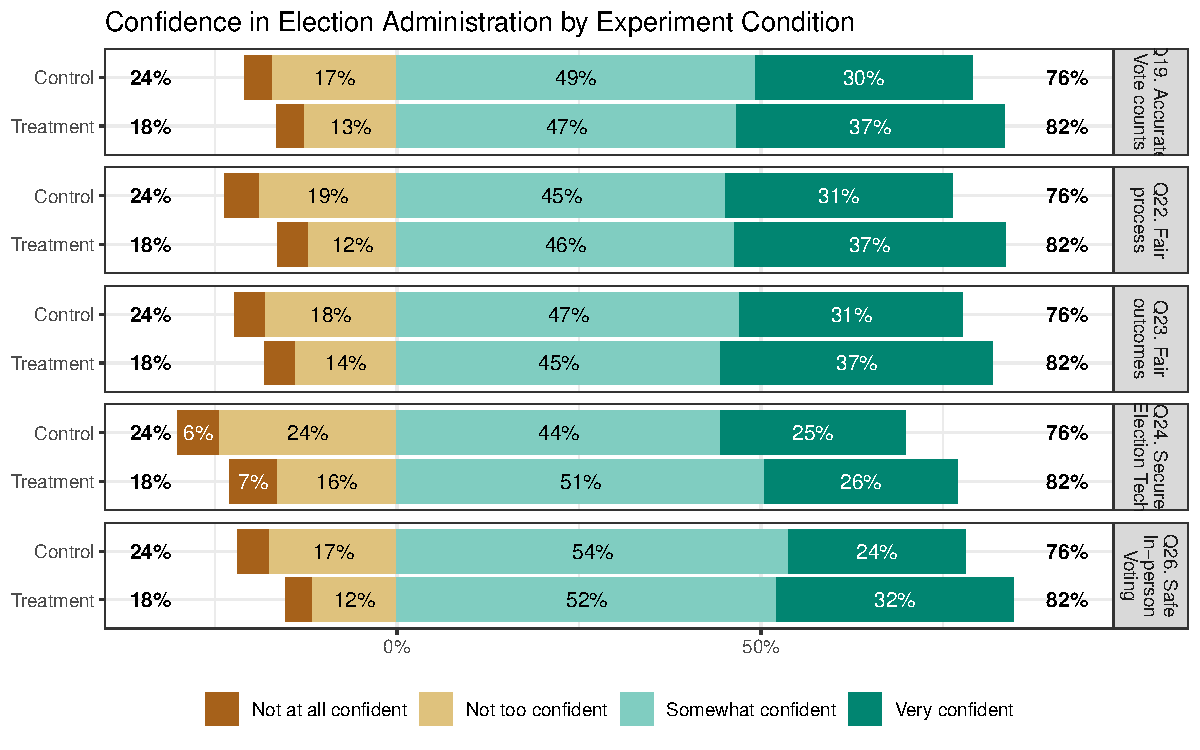
\includegraphics{index_files/figure-pdf/unnamed-chunk-7-1.pdf}

}

\caption{Confidence in Election Administration by Experiment Condition}

\end{figure}%

\newpage{}

\subsection{Survey Questions by Treatment
Condition}\label{survey-questions-by-treatment-condition}

\subsubsection{Trust and Confidence in AZ
Elections}\label{trust-and-confidence-in-az-elections}

The following cross-tables break down relative observations and
percentages of responses to survey questions across categories of the
survey's experimental condition. The survey questions in the table below
concerned a respondent's degree of trust and confidence in the electoral
process in Maricopa County, AZ.

\begin{table}

\caption{\label{tbl-1}Trust and Confidence in Maricopa County, AZ
Elections by Treatment Condition}

\centering{

\centering\begingroup\fontsize{13}{15}\selectfont

\begin{tabular}[t]{llll}
\toprule
  & Control & Treatment & P-value\\
\midrule
 & (N=624) & (N=639) & \\
\addlinespace[0.3em]
\multicolumn{4}{l}{\textbf{Confidence vote counts will be accurate, AZ}}\\
\hspace{1em}Not\_confident & 131 (21.0\%) & 106 (16.6\%) & 0.0533\\
\hspace{1em}Confident & 493 (79.0\%) & 533 (83.4\%) & \\
\addlinespace[0.3em]
\multicolumn{4}{l}{\textbf{Competence of Election Staff, AZ}}\\
\hspace{1em}Not\_confident & 129 (20.7\%) & 103 (16.1\%) & 0.0451\\
\hspace{1em}Confident & 495 (79.3\%) & 535 (83.7\%) & \\
\addlinespace[0.3em]
\multicolumn{4}{l}{\textbf{Commitment of Election Staff, AZ}}\\
\hspace{1em}not\_committed & 106 (17.0\%) & 94 (14.7\%) & 0.303\\
\hspace{1em}committed & 518 (83.0\%) & 545 (85.3\%) & \\
\addlinespace[0.3em]
\multicolumn{4}{l}{\textbf{Fair Process, AZ}}\\
\hspace{1em}Not\_confident & 148 (23.7\%) & 105 (16.4\%) & 0.00155\\
\hspace{1em}Confident & 476 (76.3\%) & 534 (83.6\%) & \\
\addlinespace[0.3em]
\multicolumn{4}{l}{\textbf{Fair Outcomes, AZ}}\\
\hspace{1em}Not\_confident & 139 (22.3\%) & 116 (18.2\%) & 0.0817\\
\hspace{1em}Confident & 485 (77.7\%) & 522 (81.7\%) & \\
\addlinespace[0.3em]
\multicolumn{4}{l}{\textbf{Security of Voting Tech, AZ}}\\
\hspace{1em}Not\_confident & 188 (30.1\%) & 147 (23.0\%) & 0.00479\\
\hspace{1em}Confident & 435 (69.7\%) & 492 (77.0\%) & \\
\addlinespace[0.3em]
\multicolumn{4}{l}{\textbf{Voters Will Be Free From Intimidation/Violence, AZ}}\\
\hspace{1em}not\_concerned & 292 (46.8\%) & 349 (54.6\%) & 0.00646\\
\hspace{1em}concerned & 332 (53.2\%) & 290 (45.4\%) & \\
\addlinespace[0.3em]
\multicolumn{4}{l}{\textbf{Safe In-person Voting, AZ}}\\
\hspace{1em}Not\_confident & 137 (22.0\%) & 98 (15.3\%) & 0.00332\\
\hspace{1em}Confident & 487 (78.0\%) & 540 (84.5\%) & \\
\addlinespace[0.3em]
\multicolumn{4}{l}{\textbf{Election Official Approval, AZ}}\\
\hspace{1em}disapprove & 160 (25.6\%) & 134 (21.0\%) & 0.0618\\
\hspace{1em}approve & 463 (74.2\%) & 502 (78.6\%) & \\
\addlinespace[0.3em]
\multicolumn{4}{l}{\textbf{Adopt AZ Program}}\\
\hspace{1em}oppose & 170 (27.2\%) & 144 (22.5\%) & 0.059\\
\hspace{1em}support & 452 (72.4\%) & 494 (77.3\%) & \\
\bottomrule
\multicolumn{4}{l}{\rule{0pt}{1em}\textit{Note: }}\\
\multicolumn{4}{l}{\rule{0pt}{1em}makecell[l]{Table reflects column percentages. \P-values based on Pearson's Chi-squared test of independence.}}\\
\end{tabular}
\endgroup{}

}

\end{table}%

\subsubsection{Expectation of Electoral
Fraud}\label{expectation-of-electoral-fraud}

The next figure and table reviews a set of questions designed to assess
a respondent's expectation of electoral fraud of some sort in Maricopa
County, AZ. Again, responses are compared across categories of the
survey experiment.

For each of the following five statements, survey participants responded
with their expectations of the likelihood that each would occur in
Maricopa County, Arizona this election cycle on a scale of ``Not likely
at all'' to ``Very likely''. The five statements were prefaced with the
question, ``How likely do you think any or all of the following will
happen during this year´s elections in Maricopa County, AZ?''

\begin{enumerate}
\def\labelenumi{\arabic{enumi}.}
\tightlist
\item
  There will be voter fraud, that is, people who are not eligible to
  vote will vote, or vote more than once;
\item
  Many votes will not actually be counted
\item
  Many people will show up to vote and be told they are not eligible
\item
  A foreign country will tamper with the votes cast in this area to
  change the results
\item
  Election officials in Maricopa County, Arizona will try to discourage
  some people from voting
\end{enumerate}

\begin{figure}

\centering{

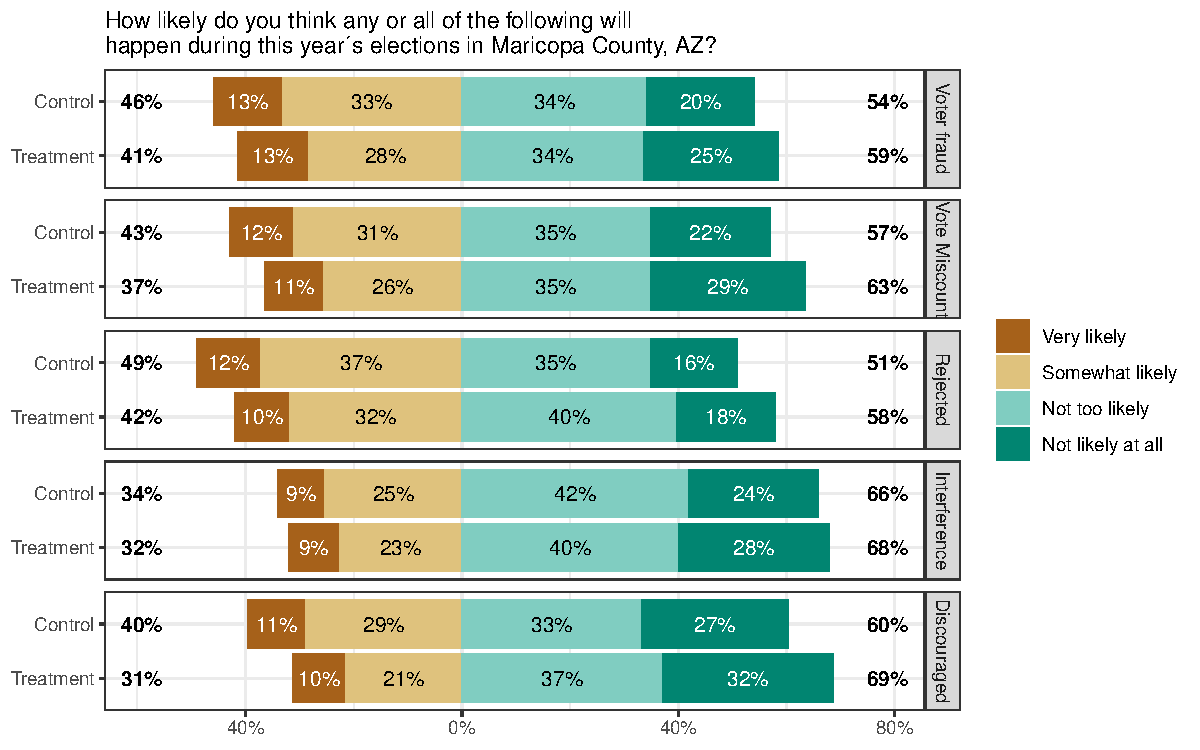
\includegraphics{index_files/figure-pdf/fig-q28-1.pdf}

}

\caption{\label{fig-q28}Expectation of Electoral Fraud in Maricopa
County, AZ by Experiment Condition}

\end{figure}%

\begin{table}

\caption{\label{tbl-2}Expectation of Electoral Fraud in Maricopa County,
AZ by Treatment Condition}

\centering{

~

Control

Treatment

P-value

(N=624)

(N=639)

Voter fraud, AZ

Not\_likely

337 (54.0\%)

374 (58.5\%)

0.126

Likely

286 (45.8\%)

265 (41.5\%)

Votes won't be counted, AZ

Not\_likely

355 (56.9\%)

405 (63.4\%)

0.0215

Likely

268 (42.9\%)

233 (36.5\%)

People will turned away, AZ

Not\_likely

317 (50.8\%)

370 (57.9\%)

0.0132

Likely

306 (49.0\%)

268 (41.9\%)

Foreign interference with votes, AZ

Not\_likely

411 (65.9\%)

434 (67.9\%)

0.499

Likely

212 (34.0\%)

205 (32.1\%)

EOs discourage people from voting, AZ

Not\_likely

376 (60.3\%)

439 (68.7\%)

0.00236

Likely

247 (39.6\%)

200 (31.3\%)

{Note: }

Table reflects column percentages. P-values based on Pearson's
Chi-squared test of independence.

}

\end{table}%

\section{3-way Crosstables}\label{way-crosstables}

\begin{tcolorbox}[enhanced jigsaw, leftrule=.75mm, title=\textcolor{quarto-callout-note-color}{\faInfo}\hspace{0.5em}{Note}, bottomrule=.15mm, breakable, colback=white, rightrule=.15mm, colframe=quarto-callout-note-color-frame, titlerule=0mm, opacityback=0, opacitybacktitle=0.6, coltitle=black, left=2mm, bottomtitle=1mm, colbacktitle=quarto-callout-note-color!10!white, toptitle=1mm, arc=.35mm, toprule=.15mm]

This section is under construction. A select number of 3-way cross
tables will be presented here.

\end{tcolorbox}

\begingroup
\setlength{\LTpost}{0mm}

\begin{longtable}{lllll}

\caption{\label{tbl-q19q7}Confidence in Accurate Vote Counts among those
who do and do not believe the 2020 election was legitimate by Treatment
Condition}

\tabularnewline

\toprule
 & \multicolumn{4}{c}{{\bfseries Q19. Vote Count Confidence for Maricopa County, AZ}\textsuperscript{\textit{1}}} \\ 
\cmidrule(lr){2-5}
Q7. Legitimacy of 2020 Election\textsuperscript{\textit{2}} & {\bfseries Not at all confident} & {\bfseries Not too confident} & {\bfseries Somewhat confident} & {\bfseries Very confident} \\ 
\midrule\addlinespace[2.5pt]
\multicolumn{5}{l}{{\bfseries Control}} \\[2.5pt] 
\midrule\addlinespace[2.5pt]
Legitimate & 1.18  (5) & 10.85 (46) & 48.35 (205) & 39.62 (168) \\ 
Not legitimate & 9.50 (19) & 30.50 (61) & 51.00 (102) & 9.00  (18) \\ 
\midrule\addlinespace[2.5pt]
\multicolumn{5}{l}{{\bfseries Treatment}} \\[2.5pt] 
\midrule\addlinespace[2.5pt]
Legitimate & 2.58 (11) & 9.39 (40) & 42.25 (180) & 45.77 (195) \\ 
Not legitimate & 6.25 (13) & 19.23 (40) & 55.77 (116) & 18.75  (39) \\ 
\bottomrule

\end{longtable}

\begin{minipage}{\linewidth}
Table reflects row percentages. NAs omitted\\
\textsuperscript{\textit{1}}Q19. How confident are you that votes in Maricopa County, AZ will be counted as voters intend in the elections this November?\\
\textsuperscript{\textit{2}}Q7.Regardless of whom you supported in the 2020 election, 
do you think Joe Biden's election as president was legitimate, or was he not legitimately elected?\\
\end{minipage}
\endgroup

\subsection{Impacts on Confidence}\label{impacts-on-confidence}

\subsubsection{Impact on confidence in fairness and accuracy of
elections}\label{impact-on-confidence-in-fairness-and-accuracy-of-elections}

The following examines survey questions that asked respondents whether
particular circumstances or election official actions would have any
impact on their confidence in the fairness and accuracy of elections.
Survey participants responded to six statements, all prefaced with the
following,

\begin{quote}
``Regardless of whether any of these are actually the case, how would
the following impact your confidence in the fairness and accuracy of
elections conducted this November?''
\end{quote}

\begin{enumerate}
\def\labelenumi{\arabic{enumi}.}
\tightlist
\item
  Election officials test every machine used in the election to ensure
  they are secure.
\item
  Election officials conduct audits of ballots after every election to
  confirm the results were accurate.
\item
  Poll watchers affiliated with the political parties or candidates
  observe the election.
\item
  Election staff and volunteers include military veterans and their
  family members from the community\footnote{Two different versions of
    this statement was presented to survey participants. Half of the
    sample read the statement as, ``Election staff and volunteers
    \emph{include} military veterans and their family members from the
    community'', whereas the other half of the sample read, ``The
    \emph{majority} of election staff and volunteers consist of military
    veterans and their family members from the community.'' No
    significant differences in responses were observed between those who
    read one version of the statement over the other. However, the same
    was done for statements number 5 and 6 which concern ``lawyers from
    the community'' and ``college students from the community''.
    Significant differences were found when comparing responses between
    the different versions of these statements. See the appendix for
    further discussion on these results.}.
\item
  Election staff and volunteers include lawyers from the community.
\item
  Election staff and volunteers include college students from the
  community.
\end{enumerate}

For each statement, survey participants responded by selecting one of
five response options:

\begin{enumerate}
\def\labelenumi{\arabic{enumi}.}
\tightlist
\item
  Decrease confidence a lot
\item
  Decrease confidence somewhat
\item
  No impact on confidence
\item
  Increase confidence somewhat
\item
  Increase confidence a lot
\end{enumerate}

The primary interest concerned whether confidence in election fairness
would increase or decreased based on the composition of election staff
and volunteers. Of particular importance are responses to the statement
which asked respondents to consider whether inclusion of military
veterans and veteran's family members as election staff and volunteers
has any impact on their confidence in the fairness and accuracy of
elections in November. In this case, significant differences were
observed between treatment and control groups.

The figure below displays a clear boost in confidence when election
staff includes veterans and family members, but most especially for
those who were in the treatment group. That is, the percentage of people
who said their confidence in election fairness would increase when
election staff includes veterans was about 11.6 percentage points higher
than those who said the same in the control group.

\subsection{Fig Q41}

\begin{figure*}

\centering{

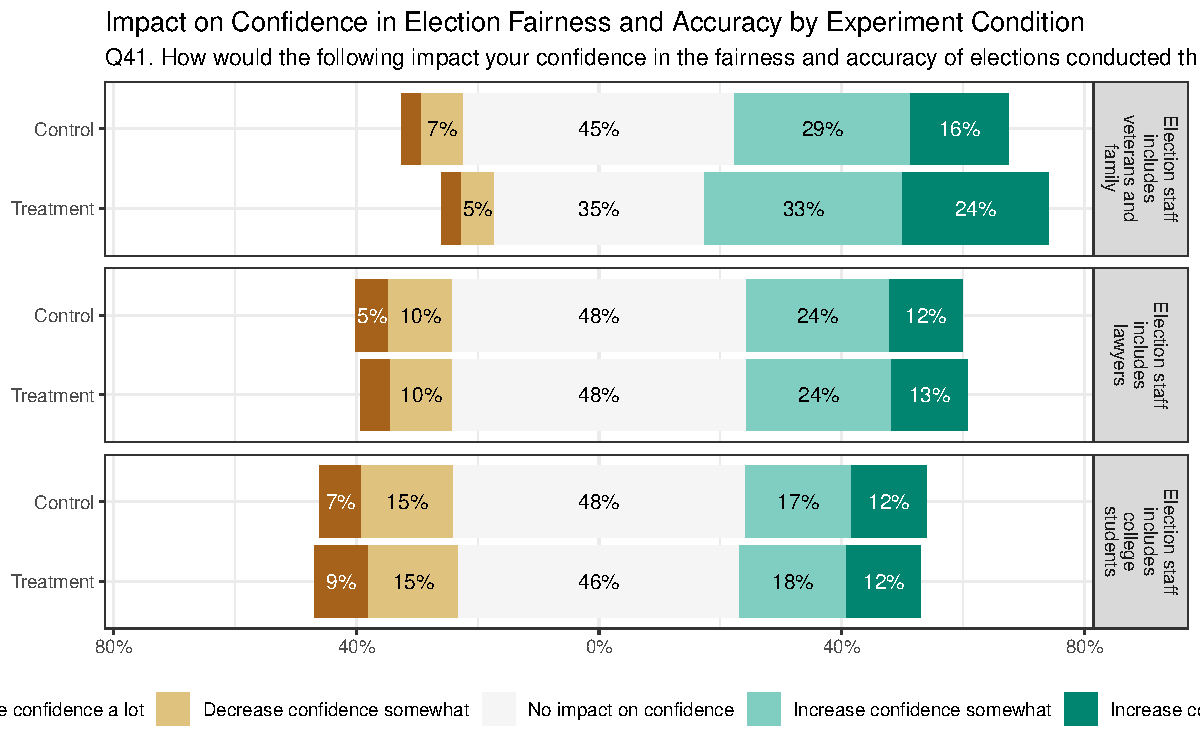
\includegraphics{index_files/figure-pdf/fig-q41-1.pdf}

}

\caption{\label{fig-q41}}

\end{figure*}%

\subsection{Q41 Coef Plot}

\begin{figure*}

\centering{

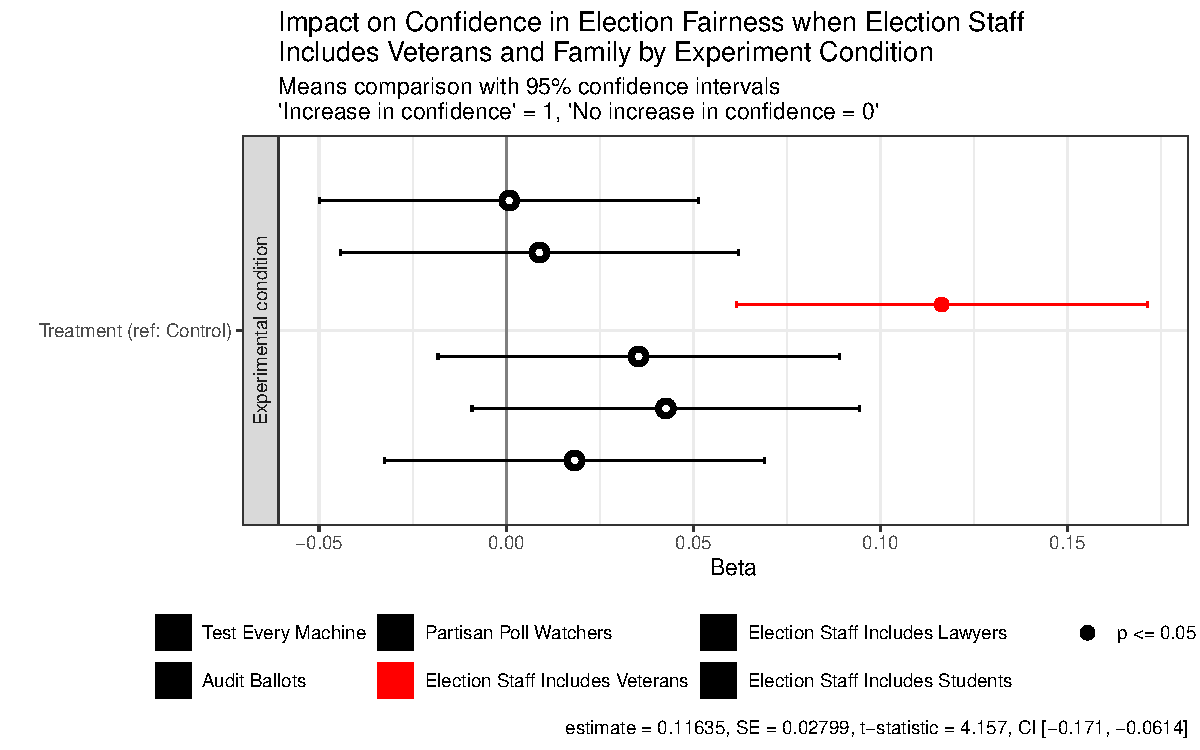
\includegraphics{index_files/figure-pdf/fig-q41-coef-plot-1.pdf}

}

\caption{\label{fig-q41-coef-plot}}

\end{figure*}%

An 11.6 percentage point difference was observed between treatment and
control groups among those who reported that their confidence in the
fairness and accuracy of elections would ``increase a lot'' or
``increase somewhat'' when election staff and volunteers include (or
consist of a majority of) military service veterans and their family
members in the community. This difference was estimated with 95\%
confidence to be statistically significant (p \textless{} 0.01, CI
{[}-0.169, -0.057{]}). Conversely, no difference was observed between
treatment and control groups among those who reported that their
confidence would ``decrease a lot'' or ``decrease somewhat''.

In the following table, responses were collapsed into three categories.
Any increase in confidence (e.g., increase confidence a lot, increase
confidence somewhat) were collapsed into one column, and likewise for
any response indicating a decrease in confidence.

\begin{table}

\caption{\label{tbl-4}Confidence Impact on Election Fairness and
Accuracy}

\centering{

\begingroup\fontsize{13}{15}\selectfont

\begin{tabu} to \linewidth {>{\raggedright}X>{\raggedright}X>{\raggedright}X>{\raggedright}X>{\raggedright}X}
\hline
Condition/Election staff include veterans and family & Decrease Confidence & No Impact & Increase Confidence & Total\\
\hline
Control & 10.11\%  (63) & 44.78\% (279) & 45.10\% (281) & 100.00\%   (623)\\
\hline
Treatment & 8.62\%  (55) & 34.64\% (221) & 56.74\% (362) & 100.00\%   (638)\\
\hline
Total & 9.36\% (118) & 39.65\% (500) & 50.99\% (643) & 100.00\% (1,261)\\
\hline
\multicolumn{5}{l}{\rule{0pt}{1em}\textit{Note: }}\\
\multicolumn{5}{l}{\rule{0pt}{1em}NA omitted. \% (n)}\\
\end{tabu}
\endgroup{}

}

\end{table}%

These results suggest that reading a vignette about county efforts to
recruit veterans as election staff and volunteers does more to increase
one's confidence in the fairness and accuracy of elections, especially
under the prospect that election staff and volunteers would include
veterans and their family members.

\subsubsection{Impact on Confidence in Voter Safety at polling
sites}\label{impact-on-confidence-in-voter-safety-at-polling-sites}

The same analysis was conducted for questions that assessed the reported
impact on confidence that voters would be safe to vote in-person. Survey
participants provided responses to the same six statements as before,
which were all prefaced with the following question,

\begin{quote}
``How would the following impact your confidence that voters are safe
from violence, threats of violence, or intimidation while voting
in-person during elections this November?''
\end{quote}

Again, the bar graph below displays a clear boost among participants in
the treatment group who reported that their confidence in voter safety
would increase when election staff is said to include veterans and their
family members.

\subsection{Fig Q43}

\begin{figure*}

\centering{

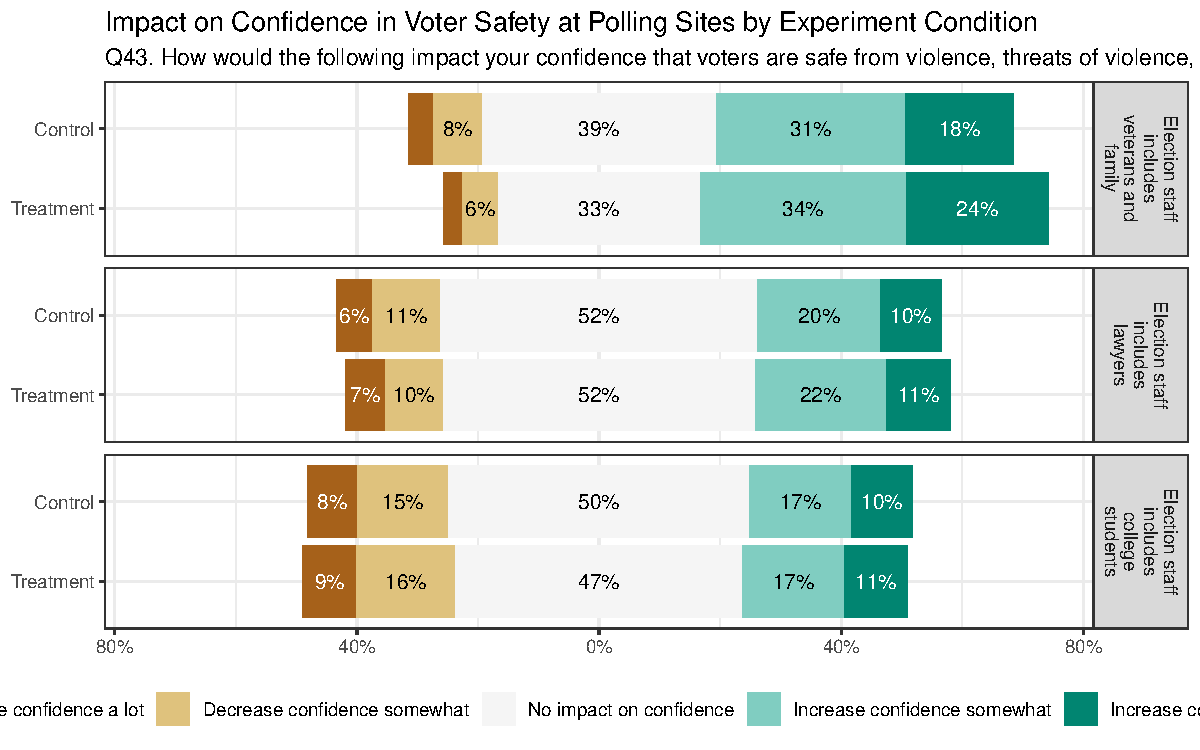
\includegraphics{index_files/figure-pdf/fig-q43-1.pdf}

}

\caption{\label{fig-q43}}

\end{figure*}%

\subsection{Q43 Coef Plot}

\begin{figure*}

\centering{

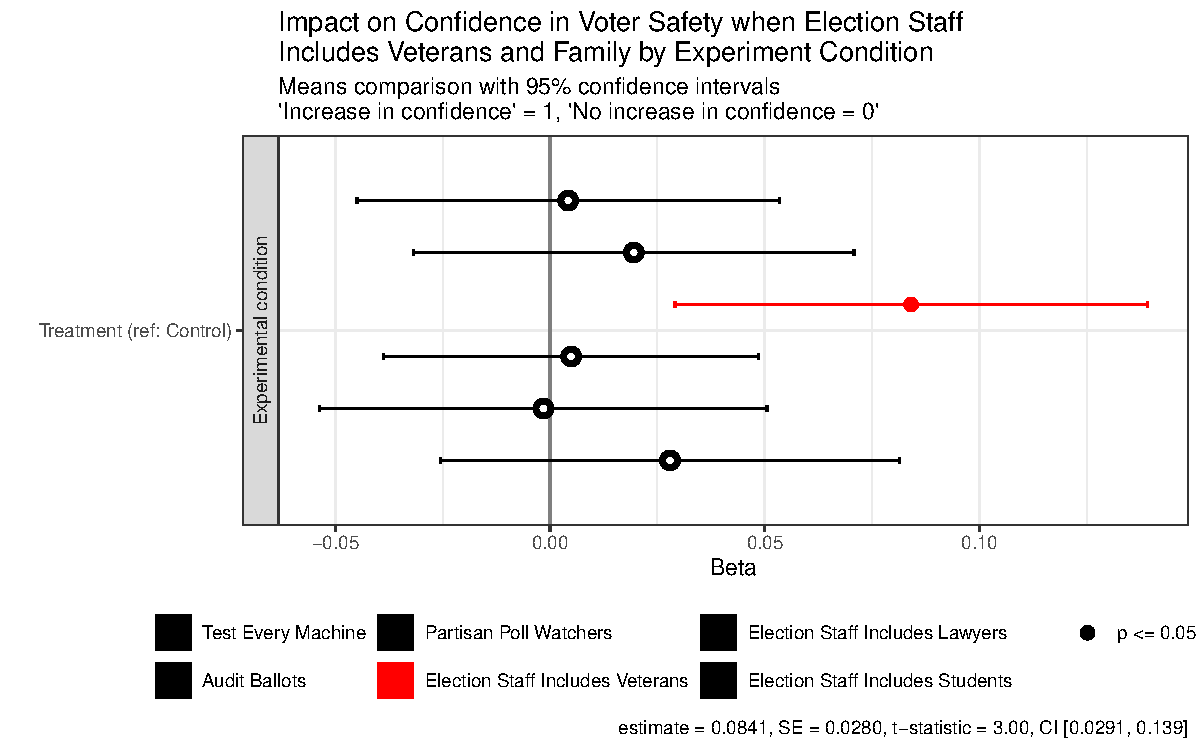
\includegraphics{index_files/figure-pdf/fig-q43-coefplot-1.pdf}

}

\caption{\label{fig-q43-coefplot}}

\end{figure*}%

The proportion of people who said their confidence in voter safety would
increase when election staff includes veterans was about 8.4 percentage
points higher than those who said the same in the control group.

\begin{table}

\caption{\label{tbl-7}Confidence Impact on In-person Voter Safety}

\centering{

\begingroup\fontsize{13}{15}\selectfont

\begin{tabu} to \linewidth {>{\raggedright}X>{\raggedright}X>{\raggedright}X>{\raggedright}X>{\raggedright}X}
\hline
Condition/Election staff include veterans and family & Decrease Confidence & No Impact & Increase Confidence & Total\\
\hline
Control & 12.20\%  (76) & 38.68\% (241) & 49.12\% (306) & 100.00\%   (623)\\
\hline
Treatment & 9.09\%  (58) & 33.39\% (213) & 57.52\% (367) & 100.00\%   (638)\\
\hline
Total & 10.63\% (134) & 36.00\% (454) & 53.37\% (673) & 100.00\% (1,261)\\
\hline
\multicolumn{5}{l}{\rule{0pt}{1em}\textit{Note: }}\\
\multicolumn{5}{l}{\rule{0pt}{1em}NA omitted. \% (n)}\\
\end{tabu}
\endgroup{}

}

\end{table}%

\section{Sample Demographics and
Balance}\label{sample-demographics-and-balance}

The decision was made to exclude any respondents who didn't complete the
survey. There were a total of 125 respondents who started but didn't
finish the survey. Of those 125, 105 quit before reaching
\texttt{Q40\_1}, whereas the rest exited the survey after that
question\footnote{Due to the programming of the survey, respondents were
  randomly assigned to either question set `A' or question set `B'. The
  grouping variable in the data set is \texttt{Qset}. Those respondents
  assigned to \texttt{Qset\ A} answered questions \texttt{Q41} and
  \texttt{Q43}; those assigned to \texttt{Qset\ B} answered question
  \texttt{Q44} and \texttt{Q46}. For each question, respondents were
  presented six statements and selected a response on a 5-point scale
  from ``Decrease Confidence a lot'' to ``Increase confidence a lot''.
  The six statements were the same for each question. This resulted in
  six variables per question within the data set (e.g., Q41\_1 to
  Q41\_6), where each variable consisted of responses to one of the six
  particular statements. Tests of differences in proportion between the
  question sets determined that responses were mostly equivalent between
  question sets (i.e., no statistically significant differences between
  proportions) except for the fifth and sixth statements pertaining to
  lawyers and college students. More detailed information on the results
  of this analysis are given in a supplementary document.}.

\texttt{NA} missing values from the \texttt{Qset} variable removes those
105 partial survey responses, i.e., respondents who quit prior to
reaching \texttt{Q40}.

\begin{table}

\caption{\label{tbl-demog}Survey sample characteristics by treatment
condition}

\centering{

\begingroup\fontsize{13}{15}\selectfont

\begin{tabu} to \linewidth {>{\raggedright}X>{\raggedright}X>{\raggedright}X>{\raggedright}X}
\toprule
  & Control & Treatment & Overall\\
\midrule
 & (N=624) & (N=639) & (N=1263)\\
\addlinespace[0.3em]
\multicolumn{4}{l}{\textbf{Age categorized into eight groups}}\\
\hspace{1em}18-24 & 56 (9.0\%) & 51 (8.0\%) & 107 (8.5\%)\\
\hspace{1em}25-34 & 107 (17.1\%) & 127 (19.9\%) & 234 (18.5\%)\\
\hspace{1em}35-44 & 130 (20.8\%) & 121 (18.9\%) & 251 (19.9\%)\\
\hspace{1em}45-54 & 113 (18.1\%) & 110 (17.2\%) & 223 (17.7\%)\\
\hspace{1em}55-64 & 124 (19.9\%) & 115 (18.0\%) & 239 (18.9\%)\\
\hspace{1em}65-74 & 70 (11.2\%) & 74 (11.6\%) & 144 (11.4\%)\\
\hspace{1em}75-84 & 20 (3.2\%) & 36 (5.6\%) & 56 (4.4\%)\\
\hspace{1em}85-92 & 4 (0.6\%) & 5 (0.8\%) & 9 (0.7\%)\\
\addlinespace[0.3em]
\multicolumn{4}{l}{\textbf{What is your current gender?}}\\
\hspace{1em}Male & 285 (45.7\%) & 307 (48.0\%) & 592 (46.9\%)\\
\hspace{1em}Female & 329 (52.7\%) & 326 (51.0\%) & 655 (51.9\%)\\
\hspace{1em}Other/Refused & 10 (1.6\%) & 6 (0.9\%) & 16 (1.3\%)\\
\addlinespace[0.3em]
\multicolumn{4}{l}{\textbf{Primary race reported by respondent}}\\
\hspace{1em}White or Caucasian & 476 (76.3\%) & 493 (77.2\%) & 969 (76.7\%)\\
\hspace{1em}Black or African American & 82 (13.1\%) & 79 (12.4\%) & 161 (12.7\%)\\
\hspace{1em}American Indian & 10 (1.6\%) & 12 (1.9\%) & 22 (1.7\%)\\
\hspace{1em}Asian & 26 (4.2\%) & 30 (4.7\%) & 56 (4.4\%)\\
\hspace{1em}Other & 30 (4.8\%) & 25 (3.9\%) & 55 (4.4\%)\\
\addlinespace[0.3em]
\multicolumn{4}{l}{\textbf{Highest level of education completed}}\\
\hspace{1em}Less than high school degree & 20 (3.2\%) & 14 (2.2\%) & 34 (2.7\%)\\
\hspace{1em}High school graduate (high school diploma or equivalent including GED) & 152 (24.4\%) & 174 (27.2\%) & 326 (25.8\%)\\
\hspace{1em}Some college but no degree & 141 (22.6\%) & 140 (21.9\%) & 281 (22.2\%)\\
\hspace{1em}Associate degree in college (2-year) & 69 (11.1\%) & 68 (10.6\%) & 137 (10.8\%)\\
\hspace{1em}Bachelor's degree in college (4-year) & 166 (26.6\%) & 156 (24.4\%) & 322 (25.5\%)\\
\hspace{1em}Master's degree & 61 (9.8\%) & 69 (10.8\%) & 130 (10.3\%)\\
\hspace{1em}Doctoral degree & 5 (0.8\%) & 13 (2.0\%) & 18 (1.4\%)\\
\hspace{1em}Professional degree (JD, MD) & 10 (1.6\%) & 5 (0.8\%) & 15 (1.2\%)\\
\addlinespace[0.3em]
\multicolumn{4}{l}{\textbf{Party ID 3 categories, with true Independents}}\\
\hspace{1em}Republican & 261 (41.8\%) & 276 (43.2\%) & 537 (42.5\%)\\
\hspace{1em}Democrat & 282 (45.2\%) & 283 (44.3\%) & 565 (44.7\%)\\
\hspace{1em}Independent & 81 (13.0\%) & 79 (12.4\%) & 160 (12.7\%)\\
\hspace{1em}Missing & 0 (0\%) & 1 (0.2\%) & 1 (0.1\%)\\
\addlinespace[0.3em]
\multicolumn{4}{l}{\textbf{Have you ever served in the Armed Forces?}}\\
\hspace{1em}Yes & 53 (8.5\%) & 68 (10.6\%) & 121 (9.6\%)\\
\hspace{1em}No & 571 (91.5\%) & 571 (89.4\%) & 1142 (90.4\%)\\
\addlinespace[0.3em]
\multicolumn{4}{l}{\textbf{Are you now serving in the Armed Forces?}}\\
\hspace{1em}Yes & 5 (0.8\%) & 10 (1.6\%) & 15 (1.2\%)\\
\hspace{1em}No & 48 (7.7\%) & 58 (9.1\%) & 106 (8.4\%)\\
\hspace{1em}Missing & 571 (91.5\%) & 571 (89.4\%) & 1142 (90.4\%)\\
\addlinespace[0.3em]
\multicolumn{4}{l}{\textbf{Member of immediate family served or is currently serving}}\\
\hspace{1em}Yes & 215 (34.5\%) & 223 (34.9\%) & 438 (34.7\%)\\
\hspace{1em}No & 409 (65.5\%) & 416 (65.1\%) & 825 (65.3\%)\\
\addlinespace[0.3em]
\multicolumn{4}{l}{\textbf{Q66. Turnout 2020}}\\
\hspace{1em}Didn't vote & 129 (20.7\%) & 117 (18.3\%) & 246 (19.5\%)\\
\hspace{1em}Unsure/Ineligible & 49 (7.9\%) & 52 (8.1\%) & 101 (8.0\%)\\
\hspace{1em}Voted & 446 (71.5\%) & 470 (73.6\%) & 916 (72.5\%)\\
\addlinespace[0.3em]
\multicolumn{4}{l}{\textbf{Who did you vote for?}}\\
\hspace{1em}Donald Trump & 214 (34.3\%) & 222 (34.7\%) & 436 (34.5\%)\\
\hspace{1em}Joe Biden & 252 (40.4\%) & 272 (42.6\%) & 524 (41.5\%)\\
\hspace{1em}Other & 30 (4.8\%) & 28 (4.4\%) & 58 (4.6\%)\\
\hspace{1em}Missing & 128 (20.5\%) & 117 (18.3\%) & 245 (19.4\%)\\
\addlinespace[0.3em]
\multicolumn{4}{l}{\textbf{Do you plan to vote?}}\\
\hspace{1em}Yes & 500 (80.1\%) & 532 (83.3\%) & 1032 (81.7\%)\\
\hspace{1em}No & 56 (9.0\%) & 54 (8.5\%) & 110 (8.7\%)\\
\hspace{1em}Undecided & 68 (10.9\%) & 53 (8.3\%) & 121 (9.6\%)\\
\bottomrule
\multicolumn{4}{l}{\rule{0pt}{1em}Table reflects column percentages.}\\
\end{tabu}
\endgroup{}

}

\end{table}%

\section{Appendix}\label{appendix}




\end{document}
